\documentclass[../body.tex]{subfiles}
\begin{document}
	
	\subsection{Выборочные коэффициенты корреляции}
	
	\begin{table}[H]
		\centering
		\begin{tabular}{| c | c | c | c |}
			\hline  \hline
			$\rho$ = 0(\ref{rho})   & $r$(\ref{r})    & $r_S$(\ref{rS}) & $r_Q$(\ref{rQ}) \\ \hline
			$E(z)$       & -0.001 & 0.002 & 0.0   \\ \hline
			$E(z^2)$     & 0.028  & 0.027 & 0.04  \\ \hline
			$D(z)$       & 0.054  & 0.055 & 0.055 \\ \hline
			$\rho$ = 0.5 & $r$    & $r_S$ & $r_Q$ \\ \hline
			$E(z)$       & 0.516  & 0.483 & 0.4   \\ \hline
			$E(z^2)$     & 0.266  & 0.233 & 0.16  \\ \hline
			$D(z)$       & 0.032  & 0.036 & 0.047 \\ \hline
			$\rho$ = 0.9 & $r$    & $r_S$ & $r_Q$ \\ \hline
			$E(z)$       & 0.906  & 0.88  & 0.8   \\ \hline
			$E(z^2)$     & 0.821  & 0.774 & 0.64  \\ \hline
			$D(z)$       & 0.002  & 0.005 & 0.029 \\
			\hline \hline
		\end{tabular}
		\caption{Двумерное нормальное распределение, n = 20}
		\label{tab:n=20}
	\end{table}

	\begin{table}[H]
		\centering
		\begin{tabular}{| c | c | c | c |}
			\hline  \hline
			$\rho$ = 0   & $r$    & $r_S$  & $r_Q$ \\ \hline
			$E(z)$       & -0.008 & -0.005 & 0.0   \\ \hline
			$E(z^2)$     & 0.009  & 0.008  & 0.004 \\ \hline
			$D(z)$       & 0.016  & 0.016  & 0.017 \\ \hline
			$\rho$ = 0.5 & $r$    & $r_S$  & $r_Q$ \\ \hline
			$E(z)$       & 0.502  & 0.481  & 0.333 \\ \hline
			$E(z^2)$     & 0.252  & 0.231  & 0.111 \\ \hline
			$D(z)$       & 0.009  & 0.01   & 0.015 \\ \hline
			$\rho$ = 0.9 & $r$    & $r_S$  & $r_Q$ \\ \hline
			$E(z)$       & 0.902  & 0.888  & 0.733 \\ \hline
			$E(z^2)$     & 0.814  & 0.788  & 0.538 \\ \hline
			$D(z)$       & 0.001  & 0.001  & 0.009 \\
			\hline \hline
		\end{tabular}
	\caption{Двумерное нормальное распределение, n = 60}
	\label{tab:n=60}
	\end{table}

	\begin{table}[H]
		\centering
		\begin{tabular}{| c | c | c | c |}
			\hline \hline
			$\rho$ = 0   & $r$    & $r_S$  & $r_Q$ \\ \hline
			$E(z)$       & -0.006 & -0.008 & 0.0   \\ \hline
			$E(z^2)$     & 0.005  & 0.005  & 0.006 \\ \hline
			$D(z)$       & 0.01   & 0.01   & 0.01  \\ \hline
			$\rho$ = 0.5 & $r$    & $r_S$  & $r_Q$ \\ \hline
			$E(z)$       & 0.499  & 0.479  & 0.32  \\ \hline
			$E(z^2)$     & 0.249  & 0.23   & 0.102 \\ \hline
			$D(z)$       & 0.005  & 0.006  & 0.009 \\ \hline
			$\rho$ = 0.9 & $r$    & $r_S$  & $r_Q$ \\ \hline
			$E(z)$       & 0.902  & 0.89   & 0.72  \\ \hline
			$E(z^2)$     & 0.813  & 0.791  & 0.518 \\ \hline
			$D(z)$       & 0.0    & 0.001  & 0.005 \\
			\hline \hline
		\end{tabular}
		\caption{Двумерное нормальное распределение, n = 100}
		\label{tab:n=100}
	\end{table}

	\begin{table}[H]
		\centering
		\begin{tabular}{| c | c | c | c |}
			\hline  \hline
			$n = 20$  & $r$   & $r_S$ & $r_Q$ \\ \hline
			$E(z)$    & 0.804 & 0.773 & 0.6   \\ \hline
			$E(z^2)$  & 0.647 & 0.597 & 0.36  \\ \hline
			$D(z)$    & 0.032 & 0.012 & 0.008  \\ \hline
			&&&\\ \hline
			$n = 60$  & $r$   & $r_S$ & $r_Q$ \\ \hline
			$E(z)$    & 0.794 & 0.771 & 0.6   \\ \hline
			$E(z^2)$  & 0.63  & 0.595 & 0.36  \\ \hline
			$D(z)$    & 0.012 & 0.004 & 0.003 \\ \hline
			&&&\\ \hline
			$n = 100$ & $r$   & $r_S$ & $r_Q$ \\ \hline
			$E(z)$    & 0.794 & 0.775 & 0.56  \\ \hline
			$E(z^2)$  & 0.63  & 0.6   & 0.314 \\ \hline
			$D(z)$    & 0.007 & 0.002 & 0.001  \\
			\hline  \hline
		\end{tabular}
		\caption{Смесь нормальных распределений}
		\label{tab:mixed}
	\end{table}

	\subsection{Эллипсы рассеивания}
	
	\begin{figure}[H]
		\centering
		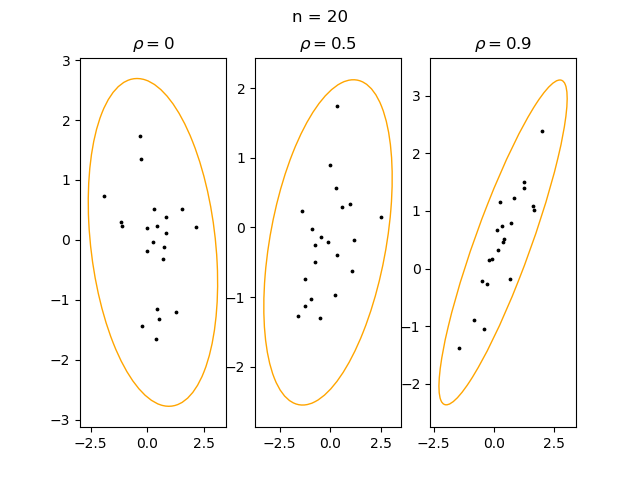
\includegraphics[width = 12cm, height = 8cm]{img/Ellipse n = 20.png}
		\caption{ Двумерное нормальное распределение, n = 20}
		\label{fig:f20}
	\end{figure}
	
	\begin{figure}[H]
		\centering
		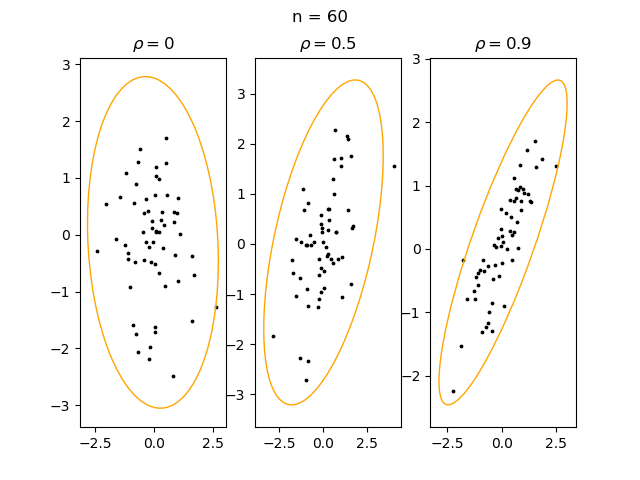
\includegraphics[width = 12cm, height = 8cm]{img/Ellipse n = 60.png}
		\caption{Двумерное нормальное распределение, n = 60}
		\label{fig:f60}
	\end{figure}
	
	\begin{figure}[H]
		\centering
		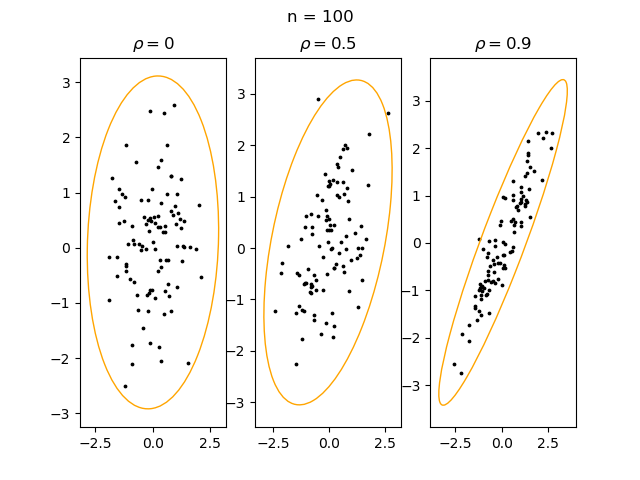
\includegraphics[width = 12cm, height = 8cm]{img/Ellipse n = 100.png}
		\caption{Двумерное нормальное распределение, n = 100}
		\label{fig:f100}
	\end{figure}
	
	\subsection{Оценки коэффициентов линейной регрессии}
	\subsubsection{Выборка без возмущений}
	\begin{itemize}
		\item Критерий наименьших квадратов: $$\hat{a}_{ls} \approx 1.86, \hat{b}_{ls} \approx 2.18$$
		\item Критерий наименьших квадратов: $$\hat{a}_{lm} \approx 1.9, \hat{b}_{lm} \approx 2.02$$
	\end{itemize}
	
	\begin{figure}[H]
		\centering
		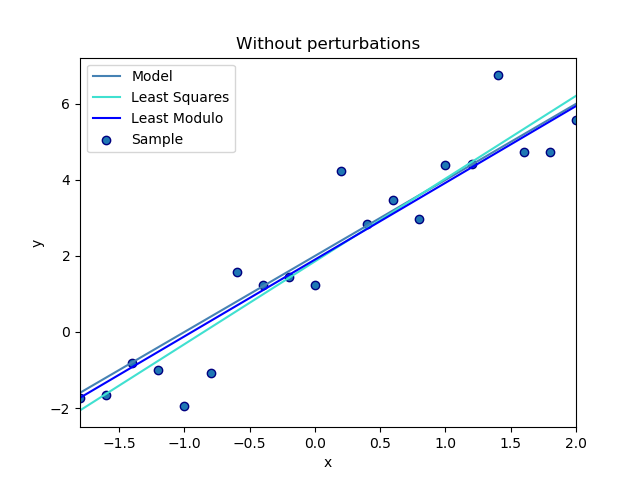
\includegraphics[width = 12cm, height = 9cm]{img/Without perturbations.png}
		\caption{Выборка без возмущений}
		\label{without}
	\end{figure}
	
	\subsubsection{Выборка с возмущениями}
	\begin{itemize}
		\item Критерий наименьших квадратов: $$\hat{a}_{ls} \approx 2.0, \hat{b}_{ls} \approx 0.77$$
		\item Критерий наименьших квадратов: $$\hat{a}_{lm} \approx 1.91, \hat{b}_{lm} \approx 1.95$$
	\end{itemize}
	
	\begin{figure}[H]
		\centering
		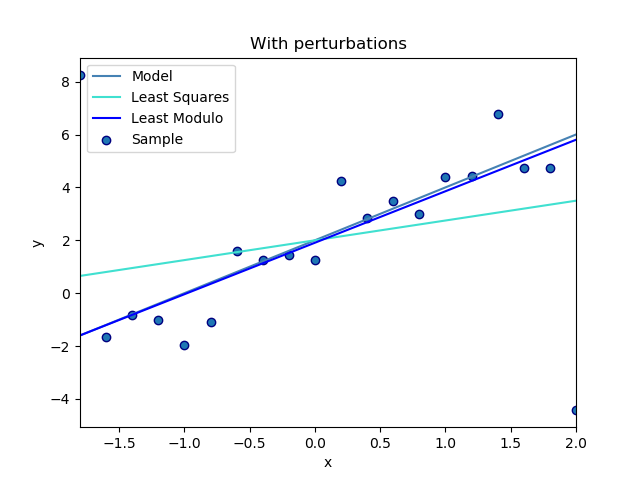
\includegraphics[width = 12cm, height = 9cm]{img/With perturbations.png}
		\caption{Выборка с возмущениями}
		\label{with}
	\end{figure}

	\subsection{Проверка гипотезы о законе распределения генеральной совокупности. Метод хи-квадрат}	
	\subsubsection{Нормальная выборка, нормальная гипотеза $H_0$.}
		Для нормального распределения согласно выведенным в примере(\ref{normal}) оценкам максимального правдоподобия:
		\begin{itemize}
			\item $\hat{\mu} = \overline{x} $
			\item $\hat{\sigma}^2 = s^2 = \frac{1}{n}\sum_{i = 1}^{n}(x_i - \overline{x})^2$
		\end{itemize}
		Тогда $\hat{\mu} \approx 0.07, \hat{\sigma} \approx 0.9$.\\ И проверяем гопотезу $H_0$, что сгенерированная по закону $N(x, 0, 1)$ $100$-элементная выборка подчиняется закону $N(x, \hat{\mu}, \hat{\sigma})$.
		Используем критерий согласия $\chi^2$:
		\begin{itemize}
			\item $\alpha = 0.05$ - уровень значимости,
			\item $n = 100$ - размер выборки,
			\item $k := \lfloor1+3.3\lg 100\rfloor = \lfloor7.6\rfloor = 7$ - количество промежутков,
			\item Квантиль $\chi_{1 - \alpha}^2(k - 1) = \chi_{0.95}^2(6) = //$ из таблицы\cite[с.~358]{math}$// \approx 12.59$
		\end{itemize}
		
		\begin{table}[H]
			\centering
			\begin{tabular}{| c | c | c | c | c | c | c |}
				\hline \hline
				&  &  &  &  &  & \\
				$i$   & $\Delta_i = [a_{i-1}, a_i)$   &   $n_i$ &   $p_i$ &   $np_i$ &   $n_i - np_i$ &   $(n_i - np_i)^2/(np_i)$ \\
				&  &  &  &  &  & \\
				\hline
				&  &  &  &  &  & \\
				1     & ($-\infty$, -1.5)           &       3 &  0.0401 &     4.01 &          -1.01 &                            0.25 \\ 
				&  &  &  &  &  & \\\hline &  &  &  &  &  & \\
				2     & [-1.5, -0.9)                &      11 &  0.0996 &     9.96 &           1.04 &                            0.11 \\ 
				&  &  &  &  &  & \\\hline &  &  &  &  &  & \\
				3     & [-0.9, -0.3)                &      16 &  0.1998 &    19.98 &          -3.98 &                            0.79 \\ 
				&  &  &  &  &  & \\\hline &  &  &  &  &  & \\
				4     & [-0.3, 0.3)                 &      33 &  0.2608 &    26.08 &           6.92 &                            1.84 \\ 
				&  &  &  &  &  & \\\hline &  &  &  &  &  & \\
				5     & [0.3, 0.9)                  &      20 &  0.2215 &    22.15 &          -2.15 &                            0.21 \\ 
				&  &  &  &  &  & \\\hline &  &  &  &  &  & \\
				6     & [0.9, 1.5)                  &      10 &  0.1224 &    12.24 &          -2.24 &                            0.41 \\ 
				&  &  &  &  &  & \\\hline &  &  &  &  &  & \\
				7     & [1.5, $+\infty$)             &       7 &  0.0559 &     5.59 &           1.41 &                            0.35 \\ 
				&  &  &  &  &  & \\\hline &  &  &  &  &  & \\
				$\sum$& ($-\infty$, $+\infty$)                           &     100 &  1      &   100    &           0    &                            3.96 = $\chi_B^2$ \\
				&  &  &  &  &  & \\\hline \hline
			\end{tabular}
			\caption{Вычисление $\chi_B^2$ при проверке гипотезы $H_0$ о нормальном законе распределения $N(x, \hat{\mu}, \hat{\sigma})$.}
			\label{chi2_normal}
		\end{table}
		Сравним $\chi_{0.95}^2(6) \approx 12.59$ и найденное  $\chi_B^2 \approx 3.96: 12.59 > 3.96.$ Следовательно гипотезу $H_0$ на данном этапе проверки можно принять.\\
		\subsubsection{Нормальная выборка, гипотеза Лапласа}
		Рассмотрим гипотезу $H_0^*$, что выборка распределена согласно закону $Laplace(x, \hat{\mu},\frac{\hat{\sigma}}{\sqrt2} )$
		Используем критерий согласия $\chi^2$:
		\begin{itemize}
			\item $\alpha = 0.05$ - уровень значимости,
			\item $n = 20$ - размер выборки,
			\item $k := \lfloor1+3.3\lg 20\rfloor = \lfloor5.3\rfloor = 5$ - количество промежутков,
			\item Квантиль $\chi_{1 - \alpha}^2(k - 1) = \chi_{0.95}^2(4) = //$ из таблицы\cite[с.~358]{math}$// \approx 9.49$
		\end{itemize}
		\begin{table}[H]
			\centering
			\begin{tabular}{| c | c | c | c | c | c | c |}
				\hline \hline
				&  &  &  &  &  & \\
				$i$   & $\Delta_i = [a_{i-1}, a_i)$   &   $n_i$ &   $p_i$ &   $np_i$ &   $n_i - np_i$ &   $(n_i - np_i)^2/np_i$ \\
				&  &  &  &  &  & \\
				\hline
				&  &  &  &  &  & \\
				1     & ($-\infty$, -1.5]           &       1 &  0.0696 &     1.39 &          -0.39 &                    0.11 \\
				&  &  &  &  &  & \\\hline &  &  &  &  &  & \\
				2     & [-1.5, -0.5)                  &       8 &  0.2499 &     5    &           3    &                    1.8  \\
				&  &  &  &  &  & \\\hline &  &  &  &  &  & \\
				3     & [-0.5, 0.5)                   &       6 &  0.5101 &    10.2  &          -4.2  &                    1.73 \\
				&  &  &  &  &  & \\\hline &  &  &  &  &  & \\
				4     & [0.5, 1.)                     &       5 &  0.1333 &     2.67 &           2.33 &                    2.04 \\
				&  &  &  &  &  & \\\hline &  &  &  &  &  & \\
				5     & [1.5, $+\infty$)            &       0 &  0.0371 &     0.74 &          -0.74 &                    0.74 \\
				&  &  &  &  &  & \\\hline &  &  &  &  &  & \\
				$\sum$  & ($-\infty$, $+\infty$)                          &      20 &  1      &    20    &           0    &                    6.43 = $\chi_B^2$ \\
				&  &  &  &  &  & \\\hline \hline
			\end{tabular}
			\caption{Вычисление $\chi_B^2$ при проверке гипотезы $H_0^*$ о $Laplace(x, \hat{\mu},\frac{\hat{\sigma}}{\sqrt2} )$.}
			\label{chi2_laplace}
		\end{table}
		Сравним $\chi_{0.95}^2(4) \approx 9.49$ и найденное  $\chi_B^2 \approx 6.43: 9.49 > 6.43.$ Следовательно гипотезу $H_0^*$ на данном этапе проверки можно принять.\\
		
		\subsection{Доверительные интервалы для параметров нормального распределения}
		\begin{table}[H]
			\centering
			\begin{tabular}{| c | c | c |}
				\hline
				n = 20   &  $m$  & $\sigma$\\ \hline
				&  -0.35 < $m$ < 0.42 & 0.63 < $\sigma$ < 1.2 \\ \hline
				&   &   \\ \hline
				n = 100   &  $m$  & $\sigma$\\ \hline
				& -0.12 < $m$ < 0.3 & 0.92 < $\sigma$ < 1.22 \\
				\hline
			\end{tabular}
			\caption{Доверительные интервалы для параметров нормального распределения}
			\label{tab:interv_simple}
		\end{table}
		
		\subsection{Доверительные интервалы для параметров нормального распределения. Асимптотический подход}
		\begin{table}[H]
			\centering
			\begin{tabular}{| c | c | c |}
				\hline
				n = 20   &  $m$  & $\sigma$\\ \hline
				& -0.32 < $m$ < 0.38 & 0.65 < $\sigma$ < 1.14 \\ \hline
				&   &   \\ \hline
				n = 100   &  $m$  & $\sigma$\\ \hline
				& -0.12 < $m$ < 0.29 & 0.93 < $\sigma$ < 1.23 \\
				\hline
			\end{tabular}
			\caption{Доверительные интервалы для параметров нормального распределения. Асимптотический подход}
			\label{tab:interv_asimpt}
		\end{table}
		
	
	
\end{document}